\documentclass[12pt,english]{scrartcl}

\usepackage{amsmath,amssymb}
%\usepackage[amssymb]{SIunits}
\usepackage{babel}
\usepackage[latin1]{inputenc}
\usepackage{graphicx}
\usepackage{color}
\usepackage[font={color=blue},figurename=Fig.,labelfont={it}]{caption}

\title{KOGW-PM-KNP: Edge detection Answers - Gaussian filtering}

\begin{document}

\maketitle
Retinal ganglion cells and neurons in the LGN respond preferentially to dark or light spots of a particular size and neurons in V1 respond preferentially to stimuli of a certain orientation and spatial frequency. Being selective to these stimulus attributes the neurons act as filters that pass some information and not other to the next level of visual information processing. This exercise will illustrate some of the transformations that are applied to the input image by neurons or filters that are selective for different features.\\
\bigskip
Work through the Python code provided and answer any following questions. 
\section*{Task 1. Gaussian filtering of an image}

 This is the equation for a 2D Gaussian, plot the output of a filter-convolved image with an appropriate $\sigma$ value.
 
\begin{enumerate}
 \item[]
 \centering
 $G(x,y) = \frac{1}{2\pi\sigma^2} e^{-\frac{x^2+y^2}{2\sigma^2}}$ \\
 \raggedright
 
 \item What happens to the image? Are these low or high-pass type filters? \\
 \item[]
 \color{blue}
 The image becomes blurred as high spatial frequency information has been filtered out. Therefore, this is a low-pass filter. 
 \color{black} 
 
 \item  Create three Gaussian filters with $\sigma$ values of 1,2 and 5. Convolve these with the input image, plot the outputs and describe them. \\
 \color{blue}
 \item[]
 As the $\sigma$, so does the blurring of the image. The greater the standard deviation of the Gaussian filter, the more high spatial frequencies are filtered (See figure below). \\
 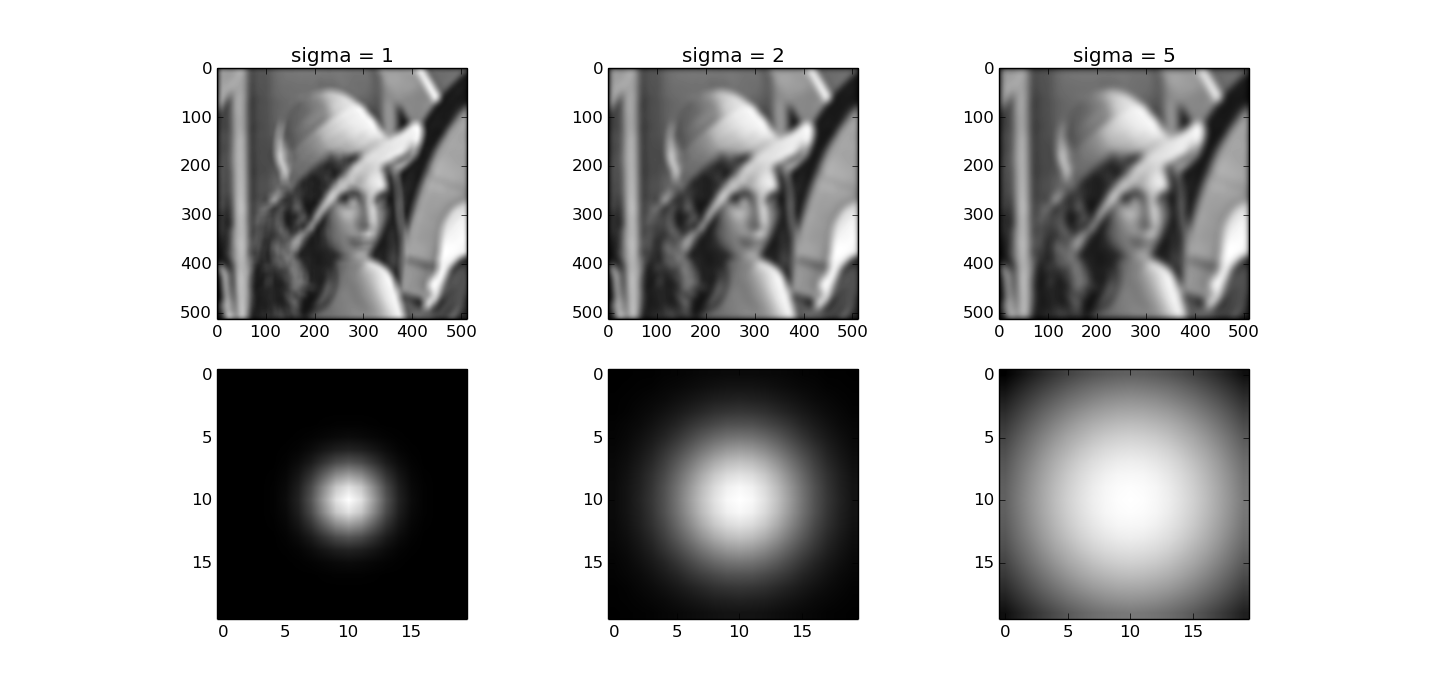
\includegraphics[scale=0.4]{../Figures/Edge_detection/Answer_T1_2.png} 
 \item[]
 
 \color{black}
 \item Can you think of a way of extracting high frequency components from an image using only a low frequency filtered image? Plot such an image and comment on its quality \\
 \item[]
 \color{blue}
 Subtract low frequency components away from original image. Thus only leaving high frequencies (or edges) as in figure below. The quality is quite poor however. \\
 \centering
 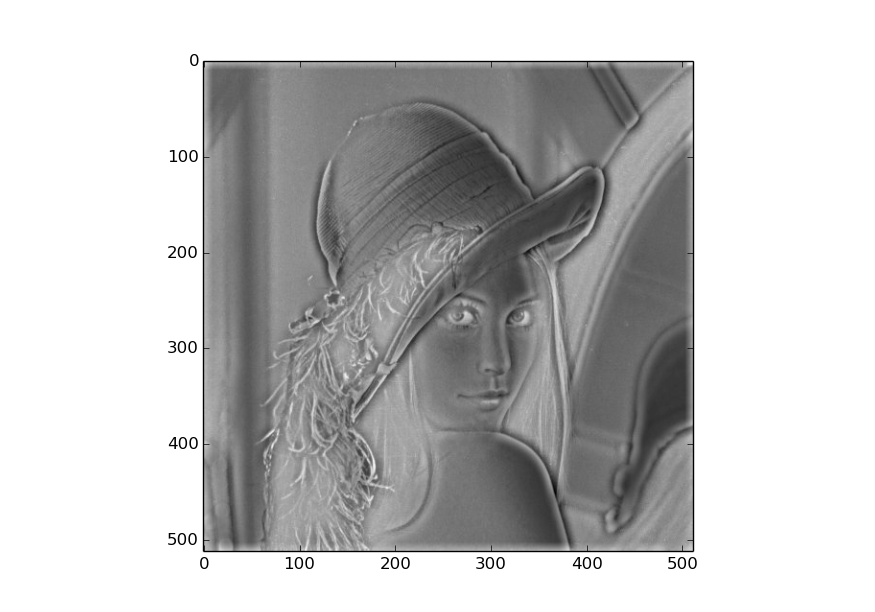
\includegraphics[scale=0.3]{../Figures/Edge_detection/Answer_T1_3.png} 
 
 \end{enumerate}


\section*{Task 2. Difference of Gaussian filtering of an image}
A Difference of Gaussian (DOG) filter is made by subtracting two different $\sigma$ valued Gaussian filters from each other. In this way, the $\sigma$ values of the filters can be used to specify which spatial frequency values are extracted.

\begin{enumerate}
 \color{black}
 \item  Read through the code. Try changing the N and $\sigma$ values. What type of filter is the DOG? Remember the two Gaussians must have different $\sigma$ values, whilst N must be the same\\ 
 \item[]
 
 \color{black}
 \item Try to find optimum $\sigma$ values for extracting edges in an image. Comment on differences between this filter and the first.\\
 \color{blue}
 Optimum filter sizes have low sigma values e.g. 1 and 2. Must be different, low values.
 \color{blue}
 Differences:
 \begin{itemize}
 \item Higher quality filter 
 \item Less image noise
 \item More easily controlled
 \end{itemize}
 
 \color{black}
 \item Try to create a DOG filter by first applying the two Gaussians to the image and then subtract the two. Is the output the same as before? \\
 \color{blue}
 Yes, virtually identical methods. Perhaps slight contrast difference.
\end{enumerate}
 

\section*{Task 3. Hybrid Images}
Using the Gaussian filter from task 1, extract low spatial frequency information from the image of Albert Einstein provided and add this to the high spatial frequency information of the Marilyn Monroe. \\
\begin{enumerate}
\item Experiment with two different sigma value Gaussian filters, until up close the combined image looks like Monroe but from afar like Einstein. \\
\color{blue} 
$\sigma$ values of 6 for Einstein and 4 for Monroe produce a good effect (N=20). \\
\color{black}
\item What does this say about the way our visual system detects images? \\
\color{blue}
That edge information dominates in object recognition. When we move further away, the edges become less clear and our brains use the broader image contents like shading. \\
\end{enumerate}


\section*{Task 4. Phase and Fourier Transforms}
\raggedright
Another way to extract image information is via the Fourier transform. Read through the code which splits the Einstein and Monroe images into their magnitude and phase components, using the Fourier transform.  \\
\bigskip
We can recombine the components for each image using the reconstruction equation below: \\
\bigskip
\centering
$Recontruction = [A(ft1)*cos(\phi(ft2))] + [A(ft1)*sin(\phi(ft2))] i$ \\
\raggedright
where A is amplitude and $\phi$ is phase.\\
\bigskip
{\it Note: i is imaginary and is denoted by "0j" in python.} \\
\bigskip
What do you notice about the output? What does this suggest about what Fourier information our visual system relies upon?

\color{blue}
In reconstruction, the phase information dominates. This suggests our brains, if using Fourier analysis, rely on phase information more than amplitude.


 
\end{document}